\chapter{Các phần cứng và sơ đồ được dùng trong đề tài} \label{phancung-sodo}
\section*{Các phần cứng} \label{phuluc-phancung}
\begin{enumerate}
\item \textit{Vi điều khiển PIC 16F887}
\begin{figure}[h]
\begin{center}
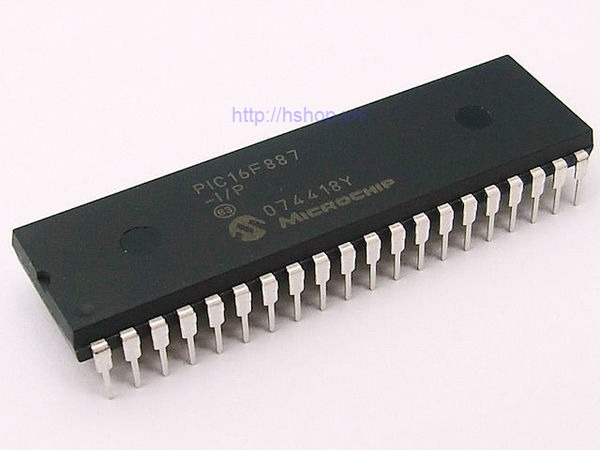
\includegraphics[scale=.3]{HW_16F887}
\end{center}
\caption{Vi điều khiển PIC 16F887}
\end{figure}

\item \textit{Cảm biến nhiệt độ DS18B20 (loại dây)}
\begin{figure}[h]
\begin{center}
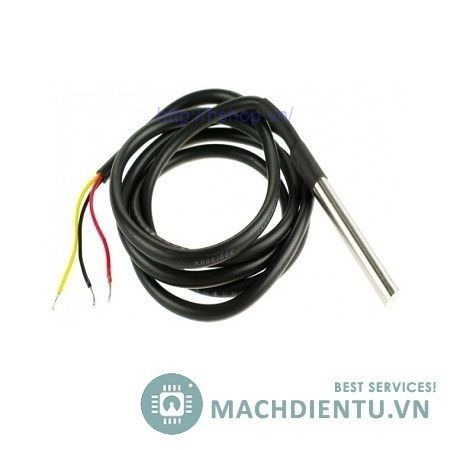
\includegraphics[scale=.3]{HW_DS18B20} 
\end{center}
\caption{Cảm biến nhiệt độ DS18B20 (loại dây)} \label{DS18B200}
\end{figure}

\item \textit{Màn hình hiển thị LCD 1602}
\begin{figure}[h]
\begin{center}
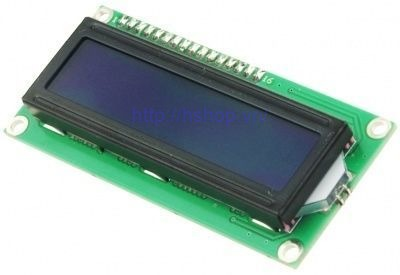
\includegraphics[scale=.35]{HW_LCD1602}
\end{center}
\caption{Màn hình hiển thị LCD 16x2} \label{LCD1602}
\end{figure}

\item \textit{Module 1 Relay với Opto cách ly kích H/L (5VDC)}
\begin{figure}[h]
\begin{center}
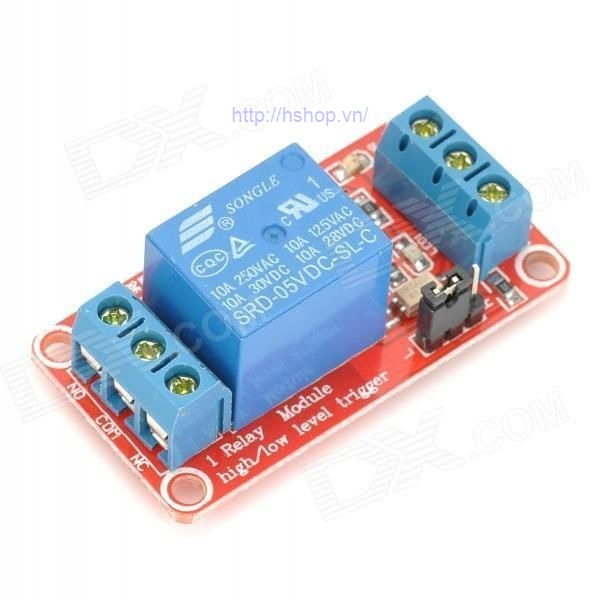
\includegraphics[scale=.2]{HW_RELAY}
\end{center}
\caption{Module Relay 5VDC với Opto cách ly}\label{RELAY}
\end{figure}

\item \textit{Mạch nạp cho vi điều khiển PIC}: mạch nạp hỗ trợ các dòng PIC: $10$, $12$, $12F$, $16C$, $16F$, $18F$.
\begin{figure}[h]
\begin{center}
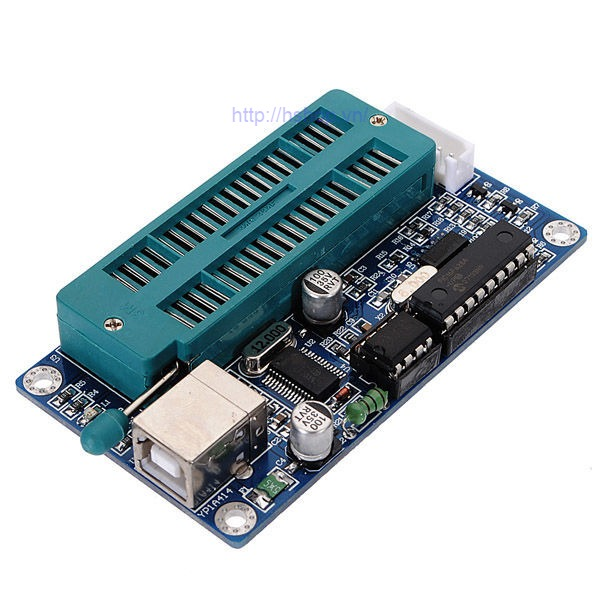
\includegraphics[scale=.25]{HW_PICKIT}
\end{center}
\caption{Mạch nạp PICKIT2 K150} 
\end{figure}
\newpage
\item \textit{Nút nhấn 4 chân}
\begin{figure}[h]
\begin{center}
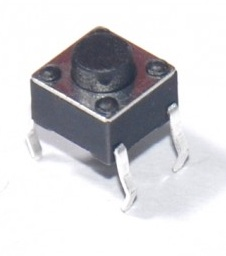
\includegraphics[scale=.3]{HW_BUTTON}
\end{center}
\caption{Nút nhấn loại 4 chân}
\end{figure}

\item \textit{Điện trở $4.7k\Omega$}
\begin{figure}[h]
\begin{center}
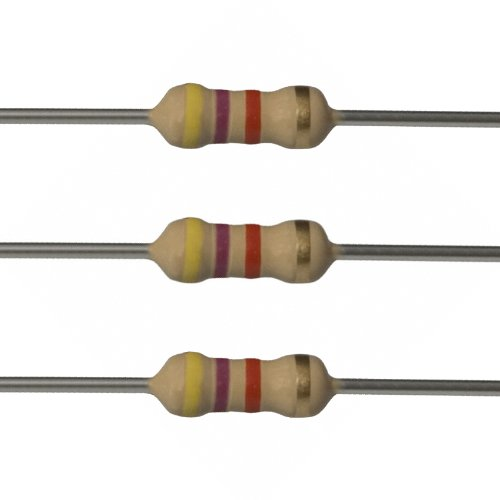
\includegraphics[scale=.2]{RES4k7}
\end{center}
\caption{Điện trở $4.7k\Omega$}
\end{figure}
\item \textit{Biến trở $10k\Omega$}
\begin{figure}[h]
\begin{center}
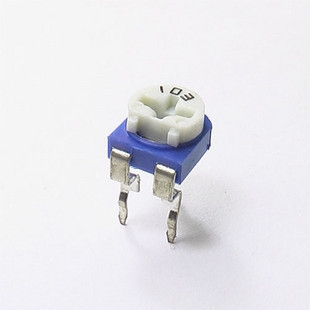
\includegraphics[scale=.3]{VAR_10k}
\end{center}
\caption{Biến trở $10k\Omega$}
\end{figure}
\newpage
\item \textit{Thạch anh tần số $20MHz$}
\begin{figure}[h]
\begin{center}
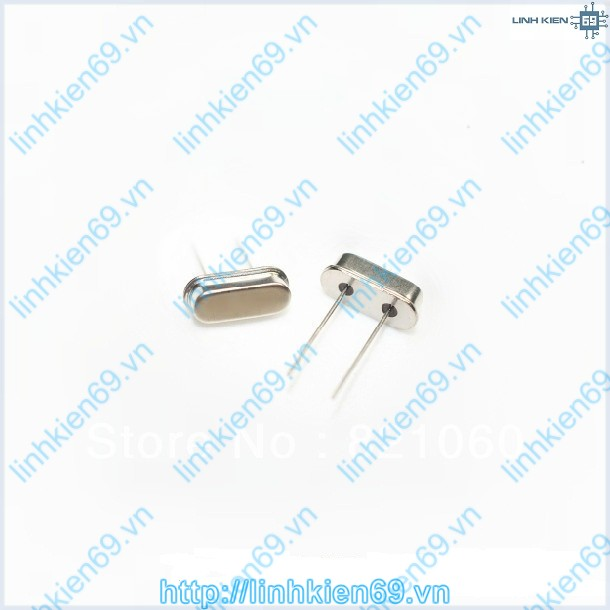
\includegraphics[scale=.15]{THACH_ANH}
\end{center}
\caption{Thạch anh tần số $20MHz$}
\end{figure}
\item \textit{Tụ điện $15pF$}
\begin{figure}[h]
\begin{center}
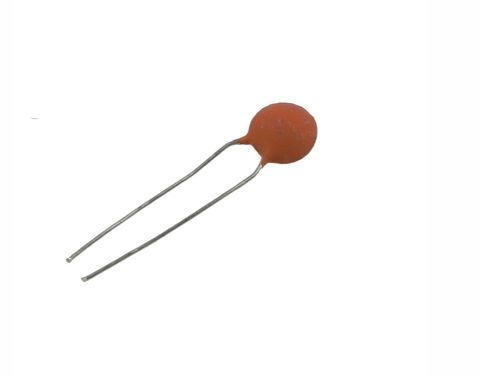
\includegraphics[scale=.5]{CAP}
\end{center}
\caption{Tụ điện $15pF$}
\end{figure}
\item \textit{Domino đấu nối loại 3 chân}
\begin{figure}[h]
\begin{center}
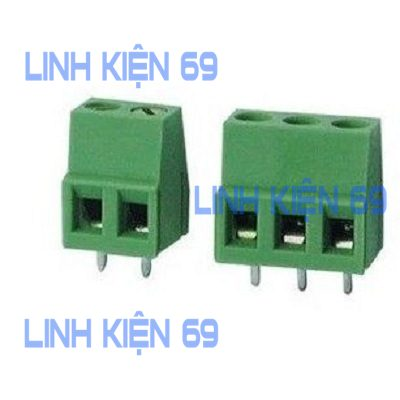
\includegraphics[scale=.4]{HW_DOMINO}
\end{center}
\caption{Domino đấu nối}
\end{figure}
\newpage
\item \textit{Đế IC 40 chân}
\begin{figure}[h]
\begin{center}
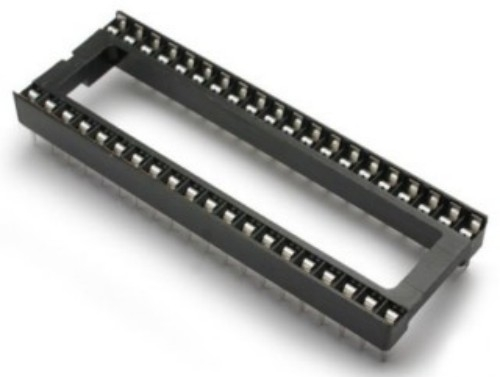
\includegraphics[scale=.3]{HW_DE_IC}
\end{center}
\caption{Đế IC 40 chân}
\end{figure}
\item \textit{Rào cái loại đơn}
\begin{figure}[h]
\begin{center}
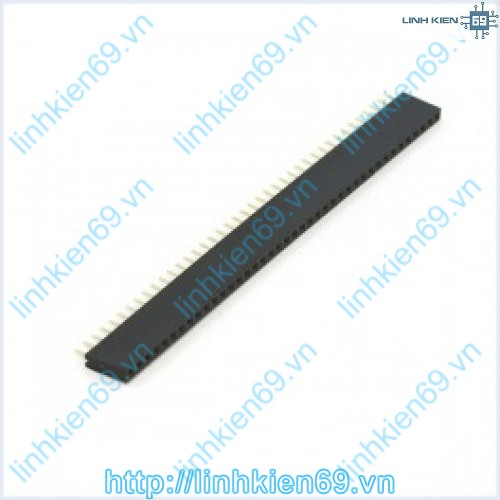
\includegraphics[scale=.25]{RAO_CAI}
\end{center}
\caption{Rào cái loại đơn}
\end{figure}
\item \textit{Rào đực loại đơn}
\begin{figure}[h]
\begin{center}
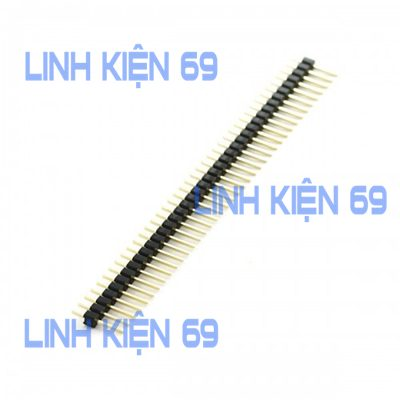
\includegraphics[scale=.35]{RAO_DUC}
\end{center}
\caption{Rào cái loại đơn}
\end{figure}
\newpage
\item \textit{Dây kết nối cái cái}
\begin{figure}[h]
\begin{center}
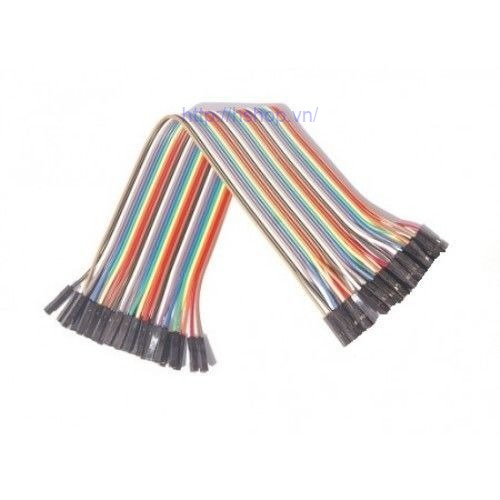
\includegraphics[scale=.3]{WIRE}
\end{center}
\caption{Dây kết nối 2 đầu cái - cái}
\end{figure}
\item \textit{Testboard hàn mạch}
\begin{figure}[h]
\begin{center}
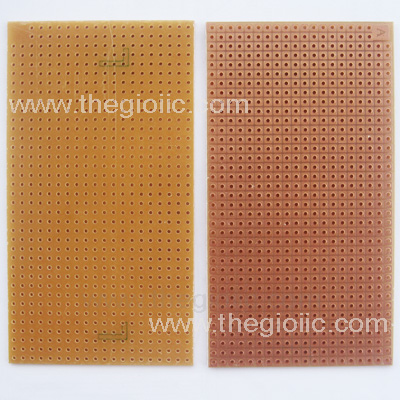
\includegraphics[scale=3]{TB_HAN}
\end{center}
\caption{Testboard hàn mạch}
\end{figure}
\item \textit{Động cơ 5VDC}
\begin{figure}[h]
\begin{center}
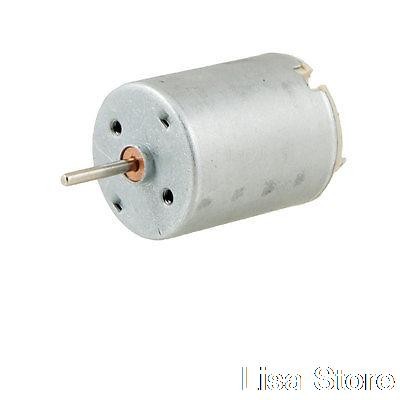
\includegraphics[scale=.3]{Motor}
\end{center}
\caption{Động cơ 5VDC}
\end{figure}
\item \textit{Bộ nguồn cấp cho vi điều khiển}: nguồn $5VDC - 2A$.
\item Các dụng cụ thực hành điện tử: VOM, mỏ hàn, chì hàn, kiềm, dây kết nối khi hàn, \ldots
\end{enumerate}